q
\chapter{Experiment Result}
\section{Experiment output}
show the result of the experiment data


is the participant experience prospective memory while doing the smartphone ?
using general data.
using all data look at the participant answer.
and look at the real fact, that how many people experience lookback.
This is shows that using while using a smartphone people experience the
prospective memory error.


\begin{table}[]
\centering
\caption{My caption}
\label{my-label}
\begin{tabular}{|l|l|l|l|l|l|l|l|l|l|}
\hline
\multirow{2}{*}{No} & \multicolumn{3}{l|}{Study 1}
                    & \multicolumn{3}{l|}{Study 2}
                    & \multicolumn{3}{l|}{Study 3}       \\ \cline{2-10}
                    & Claim that they lost intention
                    & \begin{tabular}[c]{@{}l@{}}Number of person forget the question\end{tabular}
                    & Total Person & Claim that they lost intention & Number of person forget the question&
                    Total Person & Claim that they lost intention & Number of person forget the question & Total Person \\ \hline
1                   & 0                      & 3                                                                 & 4            & 5                      & 8                       & 11           & 2                      & 2                      & 3            \\ \hline
\end{tabular}
\end{table}




\begin{figure}
\begin{center}
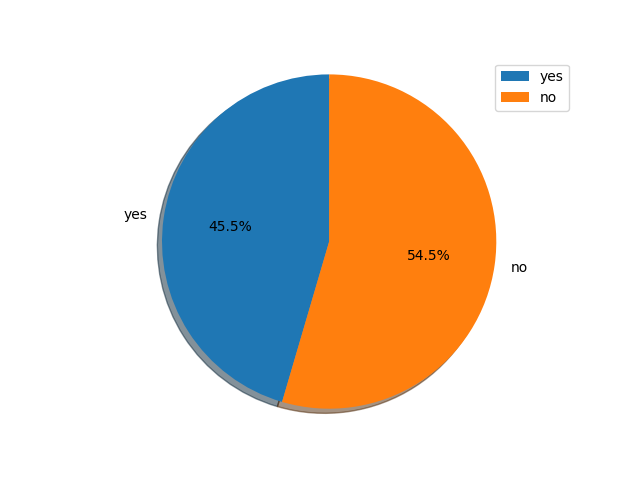
\includegraphics[scale=0.35]{demoQuestion1_study2}
\end{center}
\caption{Participant answer on the prospective memory error on smartphone (study 2)}
\label{fig:demoQuestion1_study2}
\end{figure}

so we are trying to analyze two stuff here,
one intention vs two intention



and how can the notification make people forget


and how moving from one side to another side make people harder
these three study
study 1 , average TTLFA, time_visited_answer, lookback



\begin{table}[]
\centering
\caption{My caption}
\label{my-label}
\begin{tabular}{|l|l|l|l|l|l|l|l}
\cline{1-7}
\multirow{2}{*}{Question}           & \multicolumn{2}{l|}{Study 1} & \multicolumn{2}{l|}{Study 2} & \multicolumn{2}{l|}{Study 3} &  \\ \cline{2-7}
                                    & Yes           & No           & Yes           & No           & Yes           & No           &  \\ \cline{1-7}
Experience prospective memory error & 0             & 4            & 5             & 6            & 2             & 1            &  \\ \cline{1-7}
Forget about the answer             & 2             & 2            & 4             & 7            & 0             & 3            &  \\ \cline{1-7}
\end{tabular}
\end{table}

% Please add the following required packages to your document preamble:
% \usepackage{multirow}
\begin{table}[]
\centering
\caption{My caption}
\label{my-label}
\begin{tabular}{|l|l|l|l|l|l|l|}
\hline
\multirow{2}{*}{No} & \multicolumn{3}{l|}{One Notification}                                                                                                            & \multicolumn{3}{l|}{Two Notification}                                                                                                            \\ \cline{2-7}
                    & TTFA    & \begin{tabular}[c]{@{}l@{}}time looking \\ at answer page\end{tabular} & \begin{tabular}[c]{@{}l@{}}lookback\\  frequency\end{tabular} & TTLFA   & \begin{tabular}[c]{@{}l@{}}time looking \\ at answer page\end{tabular} & \begin{tabular}[c]{@{}l@{}}lookback \\ frequency\end{tabular} \\ \hline
1                   & 7292.92 & 69517.0                                                                & 8                                                             & 7304.87 & 76699.16                                                               & 10                                                            \\ \hline
\end{tabular}
\end{table}

\section{Data analysis}
This is where I explain the result of the experiments
\section{Hypothesis testing}

\section{Discussion}
